%!TEX root = CooperBarba2014.tex

We are interested in studying the orientation of proteins near self-assembled monolayers (\sam), specifically for biosensing applications. In the framework of the implicit-solvent model, we can represent the \sam\ as a surface charge density, and use Equation \eqref{eq:matrix_dphi} to compute the electrostatic potential. 
According to the Boltzmann distribution, the probability of finding the system in micro-state $\lambda$ depends on the total free energy, $F_\text{total}$, as

\begin{equation} \label{eq:prob}
P(\lambda) = \frac{\int_{\lambda} \exp \left(-\frac{F_\text{total}}{k_B T} \right) \text{d} \lambda}{\int_{\Lambda} \exp \left(-\frac{F_\text{total}}{k_B T} \right) \text{d} \Lambda},
\end{equation} 

\noindent where $\Lambda$ is the ensemble of all micro-states, $k_B$ the Boltzmann constant and $T$ the temperature. To obtain a probability distribution, we used Equation \eqref{eq:prob} assuming that electrostatic effects were dominant, and sampled $F_\text{total}$ for different orientations. We defined the orientation using the angle between the dipole moment and surface normal vectors as a reference (tilt angle), varying from 0$^\circ$ to 180$^\circ$. Also, for each tilt angle, we rotated the protein about the dipole moment vector in 360$^\circ$ to examine all possible orientations. This process is sketched in Figure \ref{fig:1pgb_orientation}.

In this case, micro-states are defined by the tilt ($\alpha_{\text{tilt}}$) and rotational ($\alpha_{\text{rot}}$) angles, and we rewrite the integral in the numerator of Equation \eqref{eq:prob} as

\begin{equation} \label{eq:prob_angle}
\int_{\lambda} \exp \left(-\frac{F_\text{total}}{k_B T} \right) \text{d} \lambda = \int \int \exp \left(-\frac{F_\text{total}}{k_B T} \right) \text{d} \alpha_{\text{rot}} \text{d} \alpha_{\text{tilt}},
\end{equation}

\noindent where micro-state $\lambda$ is a range of angles $\alpha_{\text{rot}}$ and $\alpha_{\text{tilt}}$. 

%The study of the interaction of proteins and charged surfaces is interesting to understand how the protein orients when they are adsorbed by a surface. This is useful in biosensing applications, where the sensor surface is biofunctionalized with antibodies that bind to the target protein, and it is important that the binding sites are exposed to the flow. The most common way to place the antibodies on the sensor surface is by first functionalizing the sensor with a self-assembled monolayer (SAM) of, for example, NH$_3^+$ or COO$^-$, to which the antibody binds. This process is usually dominated by electrostatics and the surface with SAM can be represented by a surface charge density.


\begin{figure}%[h] 
   \centering
   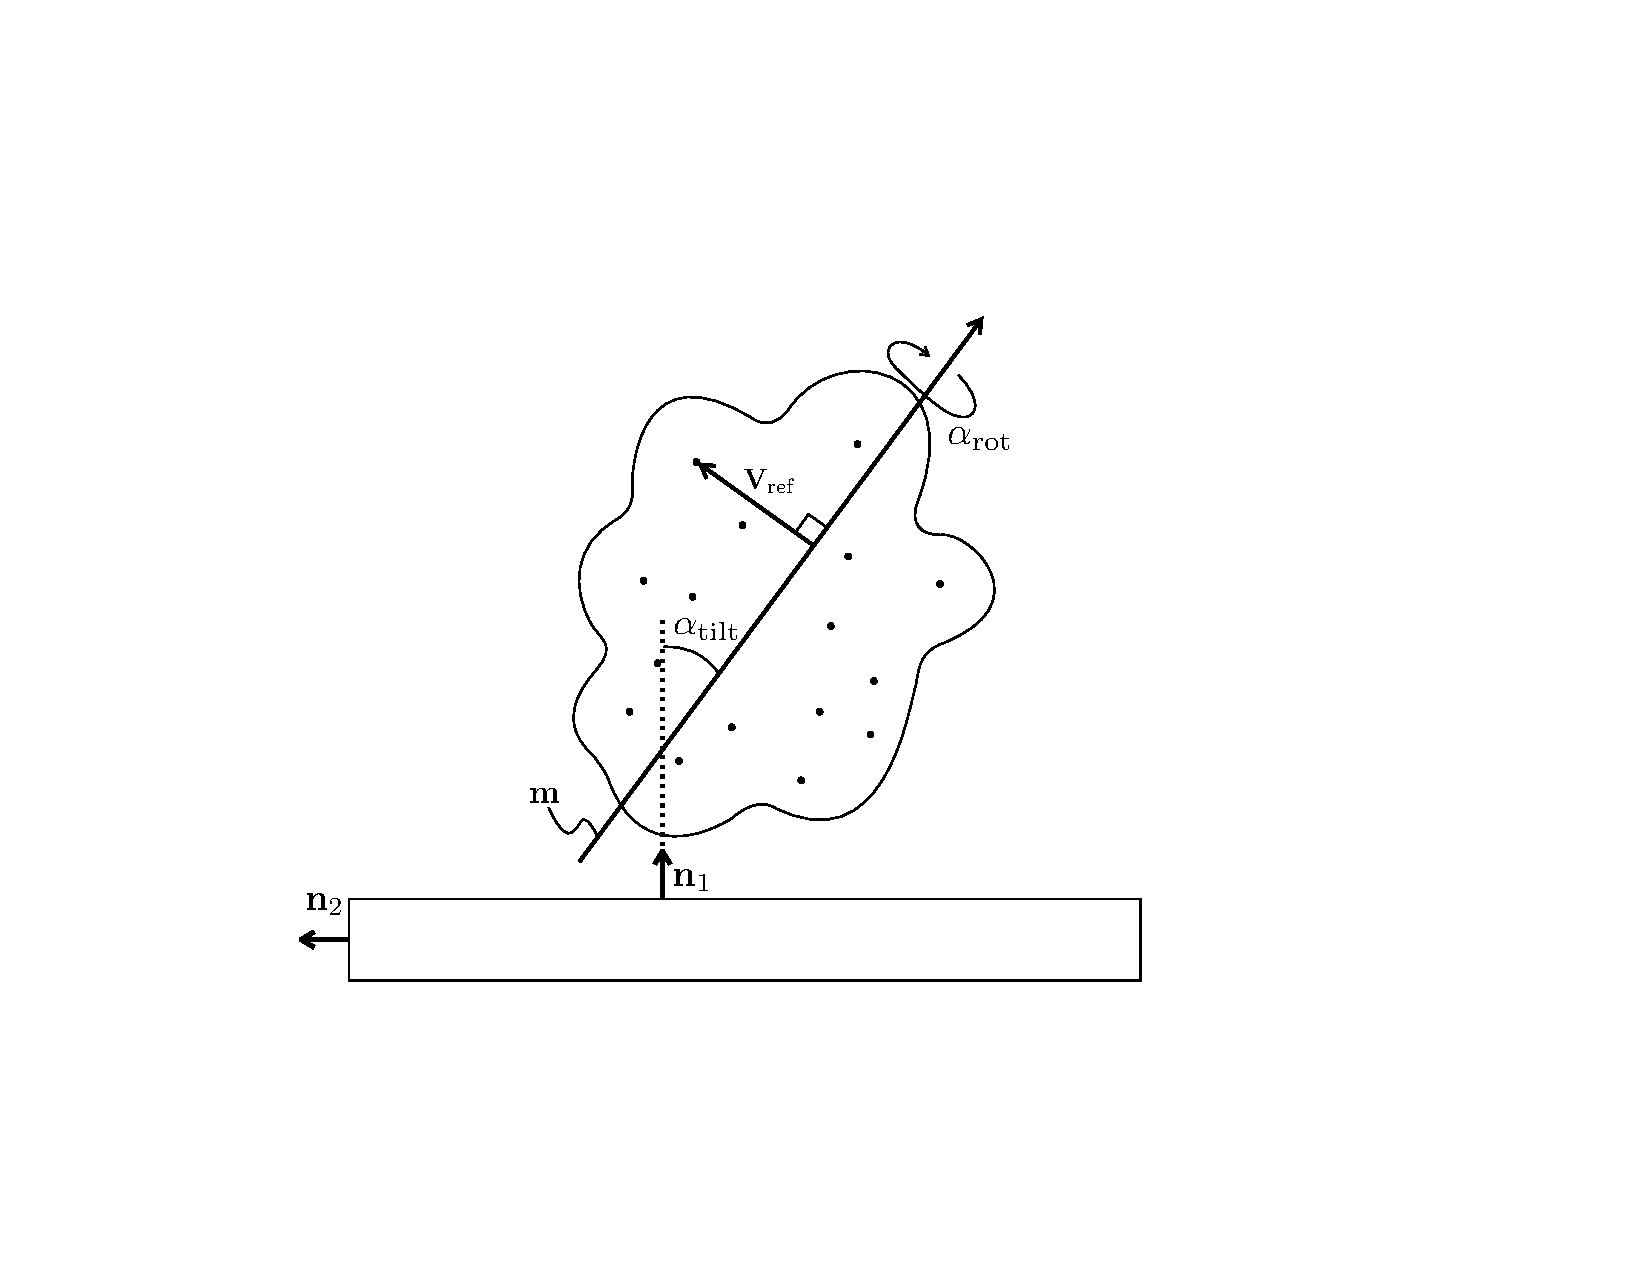
\includegraphics[width=0.5\textwidth]{Figure4.pdf}
   \caption{Setup of orientation experiment.}
   \label{fig:1pgb_orientation}
\end{figure}

To asses the performance of the implicit solvent model for investigating protein-surface interactions, we studied the orientation of protein G B1 D4$^\prime$ mutant near a charged surface, since there are molecular dynamics simulations \cite{LiuLiaoZhou2013} and experimental observations \cite{BaioWeidnerBaughGambleStaytonCastner2012} available in the literature that we could compare to. Figure \ref{fig:1pgb} shows the structure of Protein G B1 (PDB code 1PGB), to which we applied mutations E19Q, D22N, D46N and D47N to obtain the D4$^\prime$ mutant, using the SwissPdb Viewer software. \cite{GuexPeitsch1997} \footnote{\url{http://www.expasy.org/spdbv/}}

\begin{figure}%[h] 
   \centering
   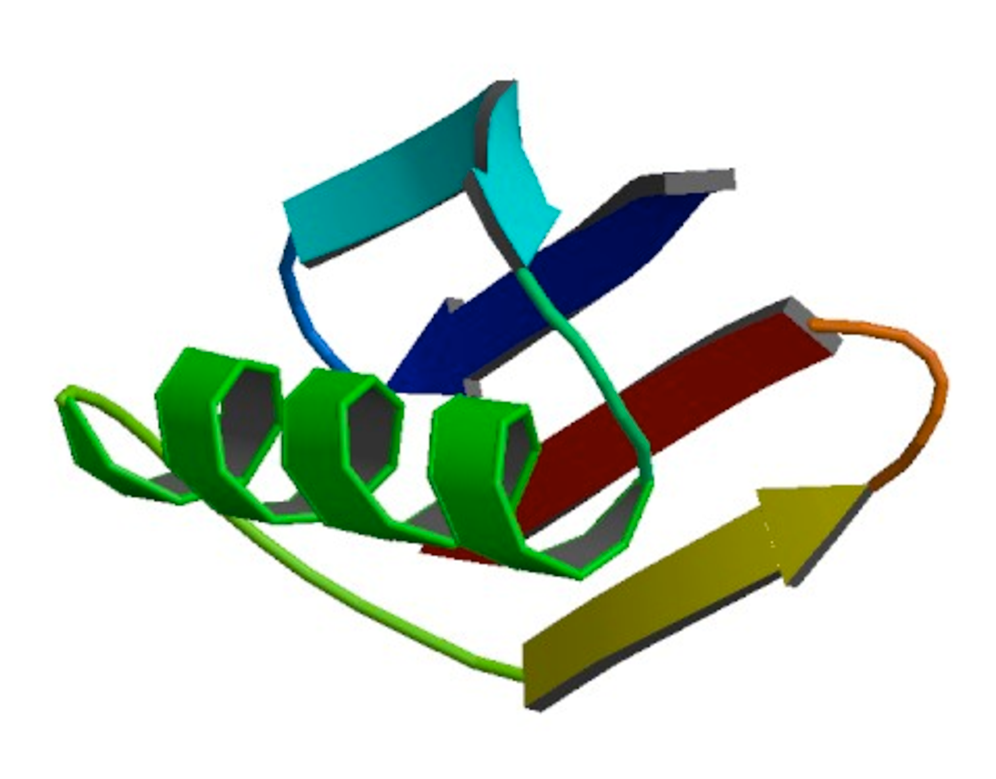
\includegraphics[width=0.25\textwidth]{Figure5.pdf}
   \caption{Structure of Protein G B1 (PDB code: 1PGB).}
   \label{fig:1pgb}
\end{figure}

We carried out a similar study for the antibody immunoglobulin G (PDB code 1IGT), a widely used protein in biosensors, whose structure is shown in Figure \ref{fig:1igt}. This is a more interesting case from the point of view of our application, yet we do not have the benefit of published simulations or experiments to compare to.

\begin{figure}%[h] 
   \centering
   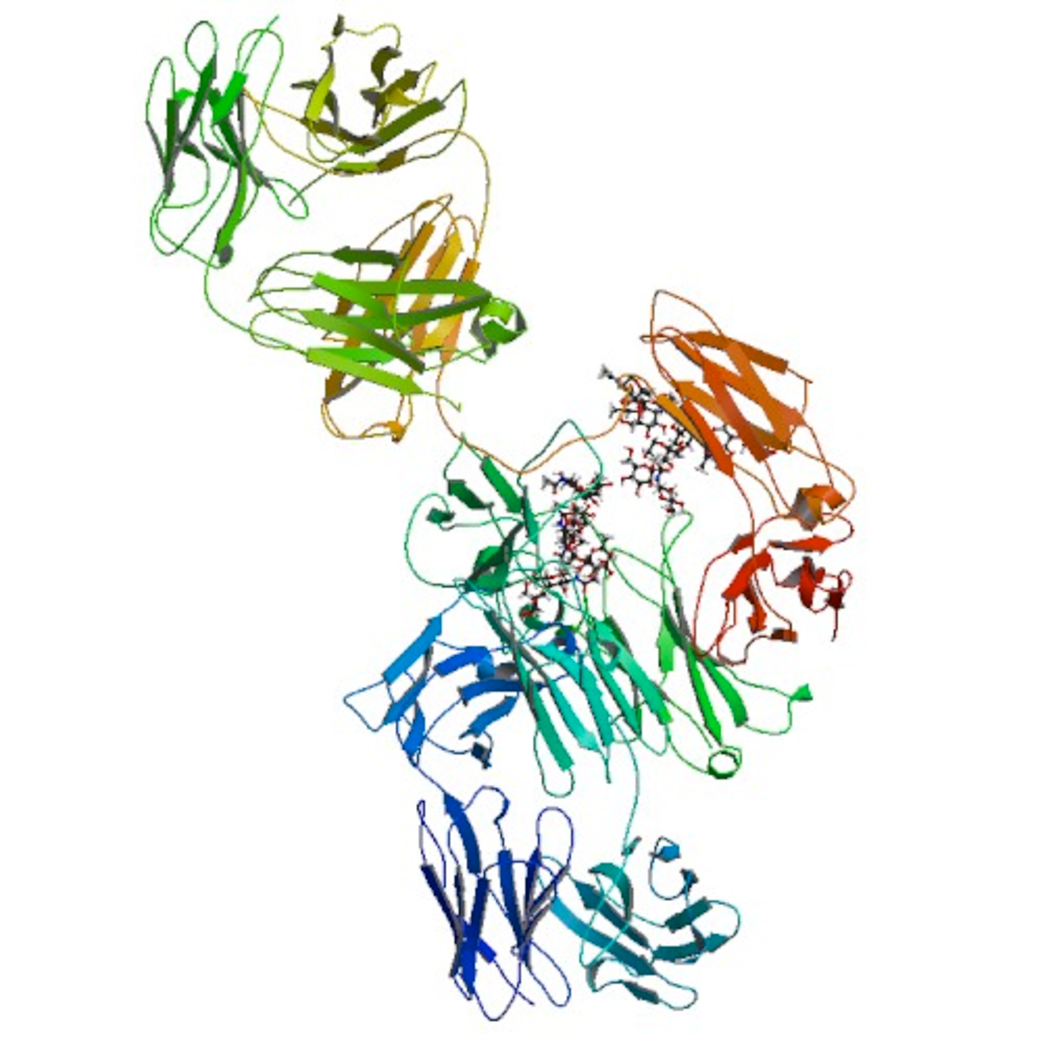
\includegraphics[width=0.35\textwidth]{Figure6.pdf}
   \caption{Structure of Immunoglobulin G (PDB code: 1IGT).}
   \label{fig:1igt}
\end{figure}

